\documentclass[12pt, a4paper]{article}
\usepackage[utf8]{inputenc}
\usepackage[T2A]{fontenc}
\usepackage[russian]{babel}
\usepackage{amsmath, amssymb}
\usepackage{graphicx}
\usepackage{geometry}
\usepackage{booktabs}
\usepackage{float}
\usepackage{hyperref}
\usepackage{caption}

\geometry{left=2cm, right=2cm, top=2cm, bottom=2cm}

\begin{document}

% ============ ТИТУЛЬНАЯ СТРАНИЦА ============
\begin{titlepage}
\centering
\vspace*{1cm}
{\small Министерство науки и высшего образования Российской Федерации\\
Федеральное государственное автономное образовательное учреждение\\
высшего образования\\
<<Национальный исследовательский университет ИТМО>>}

\vspace{2cm}
{\Large\bfseries Математическая статистика\\[0.3cm]
Расчётно-графическая работа №1}

\vspace{1cm}
{\large Описание выборки. Оценивание параметров.\\
Доверительные интервалы.}

\vspace{2cm}
\begin{flushleft}
\hspace{7cm}Выполнил: Старченко Александр\\
\hspace{7cm}Преподаватель: Ланбин Юрий Владимирович\\
\end{flushleft}

\vspace{1cm}
{\large Вариант: реальные финансовые данные РФ\\
$n = 200$}

\vfill
Санкт-Петербург, 2026
\end{titlepage}

% ============ СОДЕРЖАНИЕ ============
\tableofcontents
\newpage

% ============ ВВЕДЕНИЕ ============
\section{Данные и вариант}

Вместо синтетических данных использованы реальные финансовые данные РФ, загруженные с MOEX ISS API и сайта ЦБ РФ.

\begin{table}[H]
\centering
\caption{Описание столбцов}
\begin{tabular}{clll}
\toprule
Столбец & Данные & Источник & Распределение \\
\midrule
$X_1$ & Лог-доходности IMOEX & MOEX ISS API & $N(a, \sigma)$ \\
$X_2$ & Ставка рефинансирования ЦБ & cbr.ru/garant.ru & $Exp(\lambda, c)$ \\
$X_3$ & Копейки цены SBER & MOEX ISS API & $U(a, b)$ \\
$X_4$ & Цены IMOEX до/после 2022 & MOEX ISS API & Бимодальное \\
\bottomrule
\end{tabular}
\end{table}

\textbf{$X_1$}: 822 дневные цены закрытия IMOEX (2023--2026). Лог-доходность $r_t = \ln(P_t / P_{t-1})$. Последние 200 значений.

\textbf{$X_2$}: 140 записей ставки рефинансирования/ключевой ставки ЦБ РФ (1992--2026), пересчитанных в 411 помесячных значений (forward fill). Первые 200.

\textbf{$X_3$}: 822 цены закрытия SBER. Берётся дробная часть: $(\text{цена} \times 100) \bmod 100$. При высокой ликвидности копейки --- микроструктурный шум, распределённый $\approx$ равномерно на $[0, 99]$.

\textbf{$X_4$}: 100 цен IMOEX до кризиса 2022 ($\approx 3500$--$4200$) + 100 после ($\approx 2000$--$2500$), перемешанных случайно.

% ============ 4.1 ============
\section{Первичное описание выборки (п. 4.1)}

\subsection{Эмпирические функции распределения}

\begin{figure}[H]
\centering
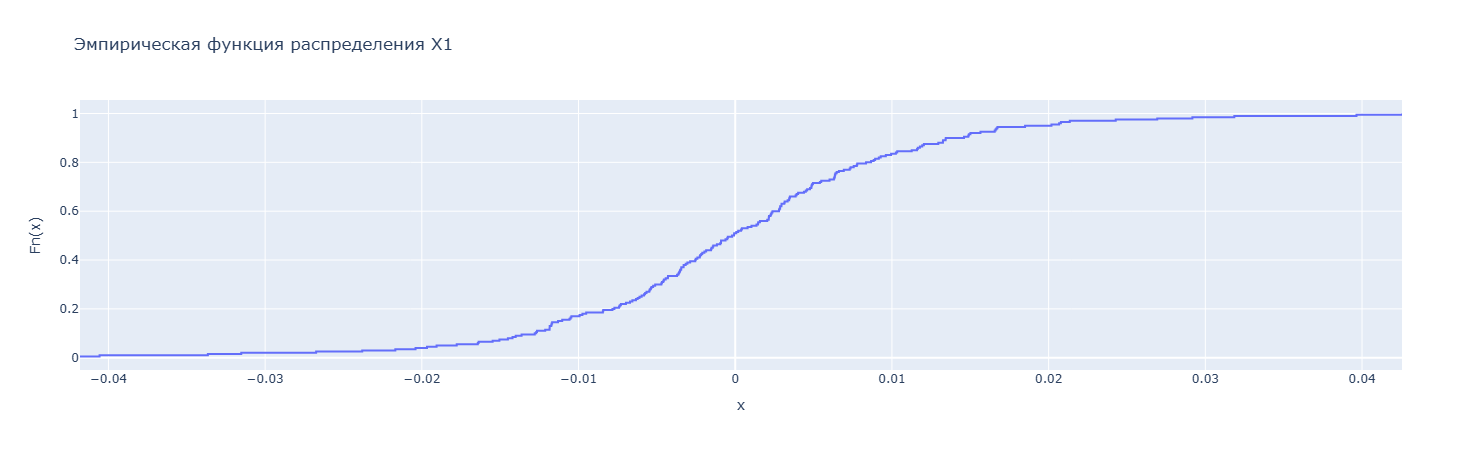
\includegraphics[width=0.85\textwidth]{plots/efr_x1.png}
\caption{ЭФР $X_1$: S-образная кривая (характерна для нормального распределения)}
\end{figure}

\begin{figure}[H]
\centering
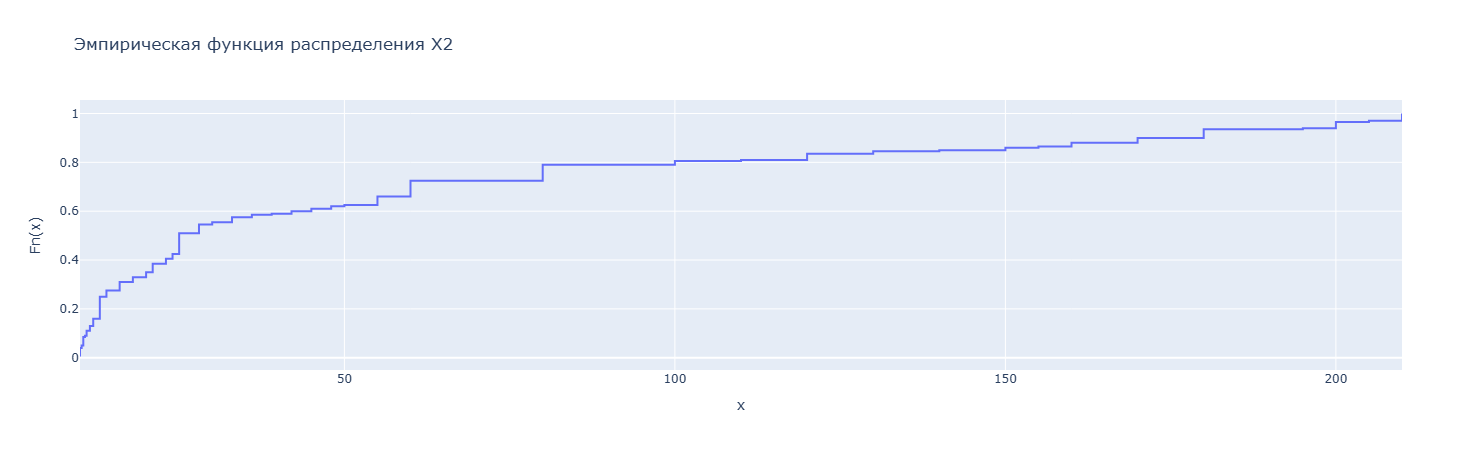
\includegraphics[width=0.85\textwidth]{plots/efr_x2.png}
\caption{ЭФР $X_2$: быстрый рост вначале, замедление --- выпуклая форма (экспоненциальное)}
\end{figure}

\begin{figure}[H]
\centering
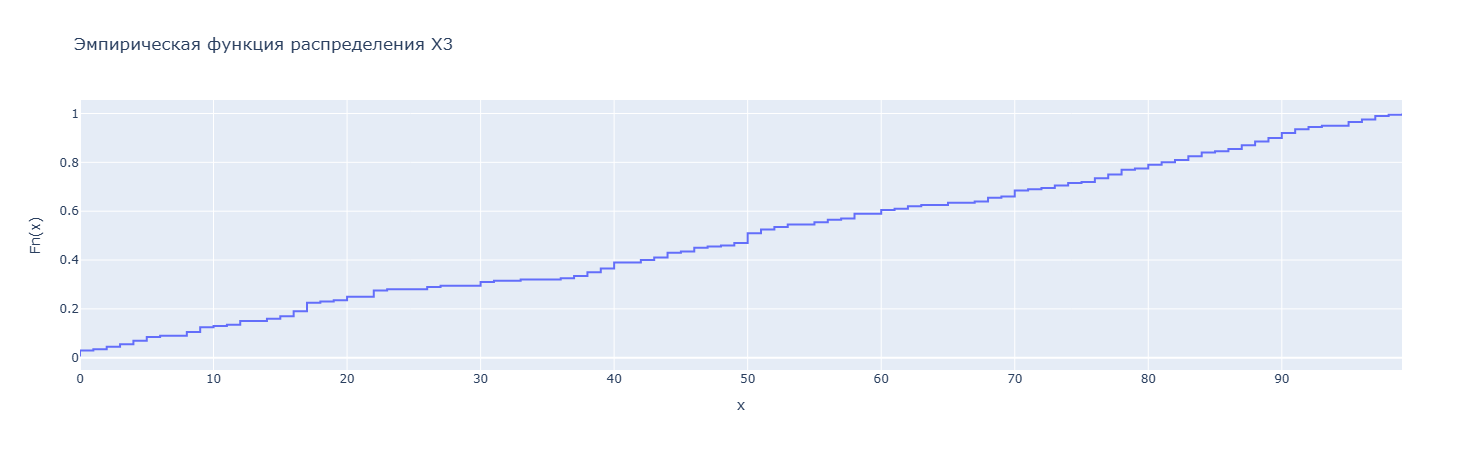
\includegraphics[width=0.85\textwidth]{plots/efr_x3.png}
\caption{ЭФР $X_3$: почти прямая линия (равномерное распределение)}
\end{figure}

\subsection{Гистограммы}

Для каждого столбца построены гистограммы по трём правилам: Стёрджес ($k = 1 + \lfloor \log_2 n \rfloor$), Скотт ($h = 3.5 \hat\sigma n^{-1/3}$), Фридман-Диаконис ($h = 2 \cdot IQR \cdot n^{-1/3}$).

\begin{figure}[H]
\centering
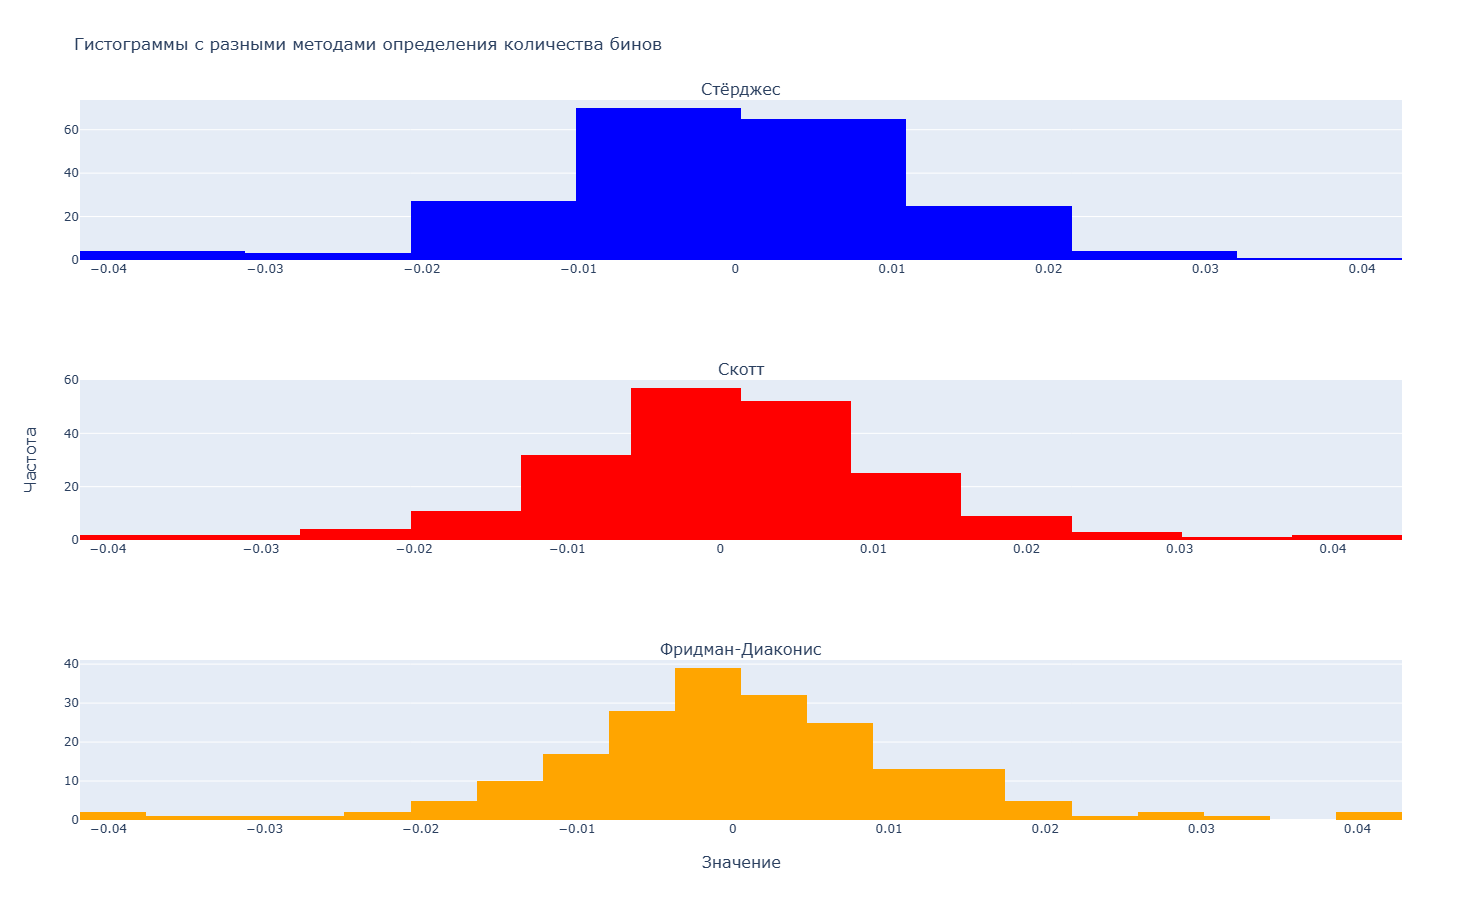
\includegraphics[width=\textwidth]{plots/hist_x1.png}
\caption{Гистограммы $X_1$: колоколообразная форма}
\end{figure}

\begin{figure}[H]
\centering
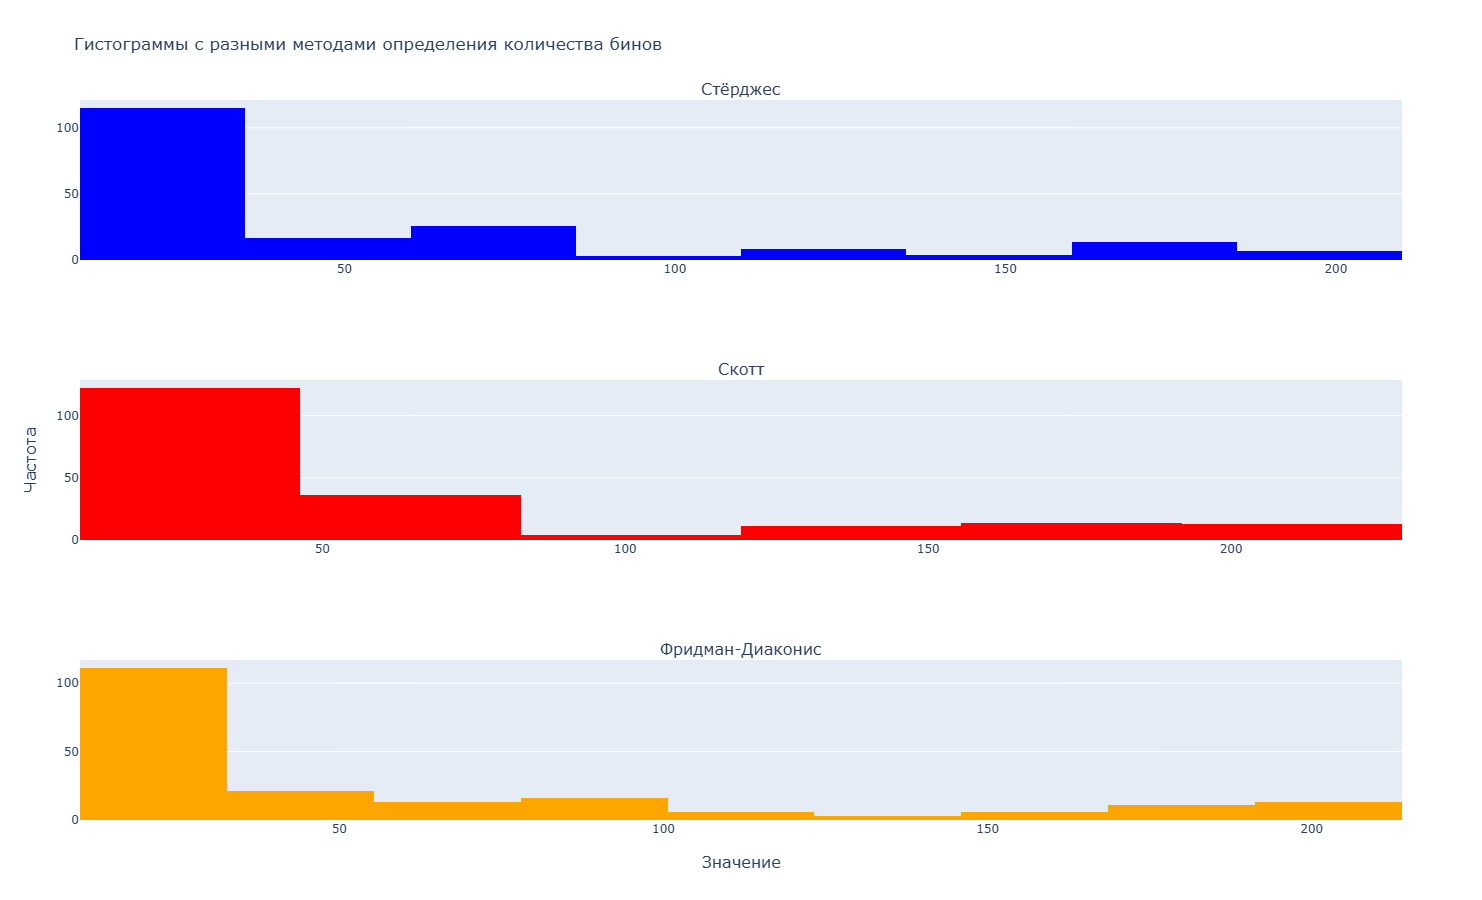
\includegraphics[width=\textwidth]{plots/hist_x2.png}
\caption{Гистограммы $X_2$: правая асимметрия, длинный хвост}
\end{figure}

\begin{figure}[H]
\centering
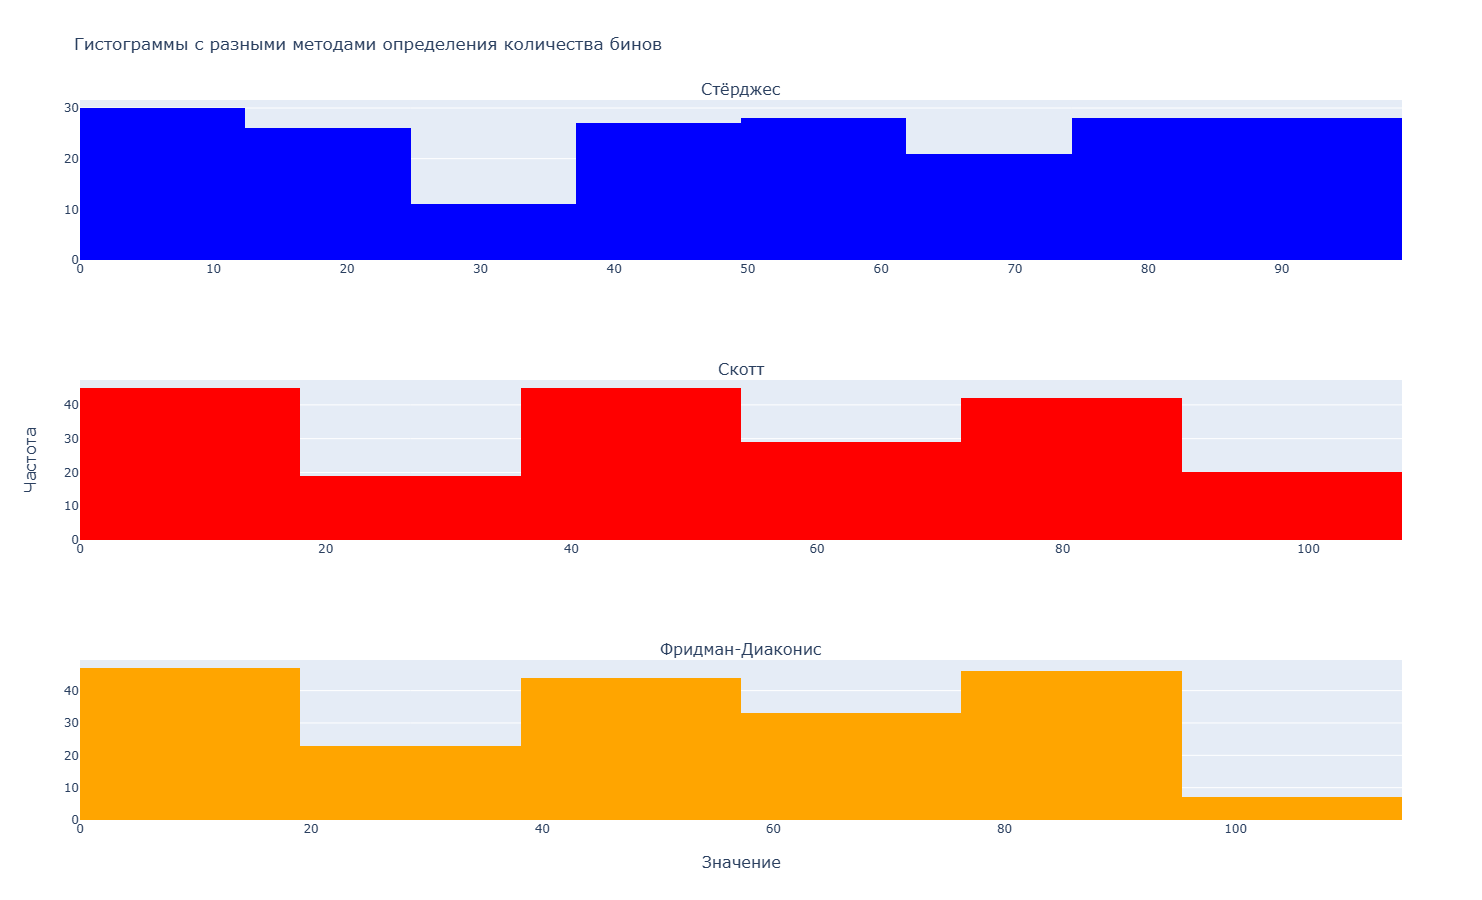
\includegraphics[width=\textwidth]{plots/hist_x3.png}
\caption{Гистограммы $X_3$: плоская форма}
\end{figure}

\subsection{Числовые характеристики}

\begin{table}[H]
\centering
\caption{Числовые характеристики выборки}
\begin{tabular}{lccc}
\toprule
Характеристика & $X_1$ & $X_2$ & $X_3$ \\
\midrule
$\bar{x}$ & $0.000071$ & $58.22$ & $50.02$ \\
$S^2$ (смещённая) & $0.000144$ & $3673.62$ & $893.68$ \\
$\hat\sigma^2$ (несмещённая) & $0.000145$ & $3692.08$ & $898.18$ \\
$S$ & $0.01199$ & $60.61$ & $29.89$ \\
$\hat\sigma$ & $0.01202$ & $60.76$ & $29.97$ \\
Медиана & $-0.00014$ & $25.0$ & $50.0$ \\
$Q_1$ & $-0.006$ & $13.75$ & $21.5$ \\
$Q_3$ & $0.006$ & $80.0$ & $77.25$ \\
\bottomrule
\end{tabular}
\end{table}

\subsection{Описание формы}

\textbf{$X_1$}: симметричное распределение ($\text{skew} = -0.01$), выбросы отсутствуют, естественных границ нет --- лог-доходности теоретически от $-\infty$ до $+\infty$.

\textbf{$X_2$}: выраженная правая асимметрия ($\text{skew} = 1.34$), присутствуют выбросы в области высоких ставок (90-е годы), естественная нижняя граница (ставка $\geq 0$).

\textbf{$X_3$}: симметричное ($\text{skew} = -0.10$), выбросы отсутствуют, естественные границы слева (0) и справа (99).

% ============ 4.2 ============
\section{Предположение о виде закона распределения (п. 4.2)}

$X_1$: колоколообразная гистограмма, S-образная ЭФР, медиана $\approx$ среднее, квартили симметричны $\Rightarrow$ \textbf{нормальное $N(a, \sigma)$}.

$X_2$: правая асимметрия, выпуклая ЭФР, медиана $\ll$ среднее, нижняя граница $\approx 10\%$ $\Rightarrow$ \textbf{экспоненциальное со сдвигом $Exp(\lambda, c)$}.

$X_3$: плоская гистограмма, линейная ЭФР, среднее = медиана = середина диапазона $\Rightarrow$ \textbf{равномерное $U(a, b)$}.

% ============ 4.3 ============
\section{Оценивание параметров (п. 4.3)}

\subsection{$X_1$: нормальное $N(a, \sigma)$}

\textbf{Метод моментов:} $EX = a$, $DX = \sigma^2$ $\Rightarrow$ $\hat a = \bar x = 0.000071$, $\hat\sigma = S = 0.01199$.

\textbf{ММП:} $L(\mu, \sigma^2) = \prod_{i=1}^{n} \frac{1}{\sqrt{2\pi}\sigma} \exp\left(-\frac{(x_i - \mu)^2}{2\sigma^2}\right)$

После дифференцирования $\ln L$: $\hat\mu = \bar x$, $\hat\sigma^2 = S^2$. Совпадает с ММ.

\subsection{$X_2$: экспоненциальное со сдвигом $Exp(\lambda, c)$}

Плотность: $f(x) = \lambda e^{-\lambda(x-c)}$, $x \geq c$. Теория: $EX = c + 1/\lambda$, $DX = 1/\lambda^2$.

\begin{figure}[H]
\centering
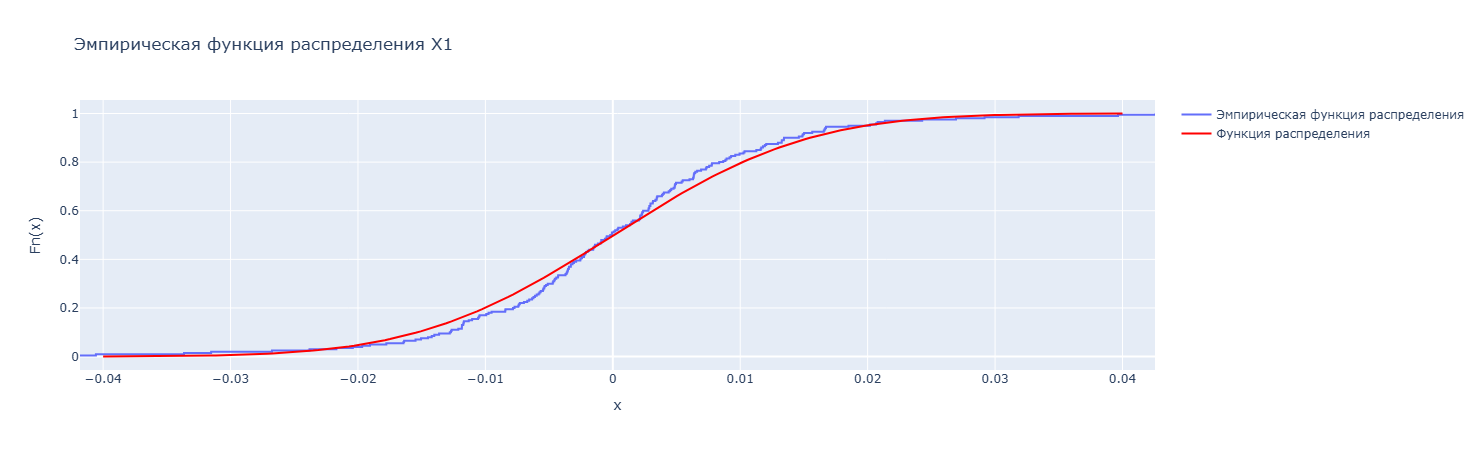
\includegraphics[width=0.85\textwidth]{plots/fit_x1.png}
\caption{$X_2$: сравнение ЭФР с теоретическими ФР, которые совпали}
\end{figure}

\textbf{Метод моментов:} $\hat\lambda_{MM} = 1/S$, $\hat c_{MM} = \bar x - 1/\hat\lambda = \bar x - S$.

\textbf{ММП:} $L(\lambda, c) = \lambda^n \exp\left(-\lambda \sum(x_i - c)\right)$ при $c \leq \min(x_i)$.

По $c$: $\partial\ln L/\partial c = n\lambda > 0$ --- растёт, значит $\hat c = \min(x_i)$.

По $\lambda$: $\hat\lambda = 1/(\bar x - \hat c)$.

Оценки различаются: ММ оценивает сдвиг через среднее и дисперсию, ММП --- через минимум выборки.

\begin{figure}[H]
\centering
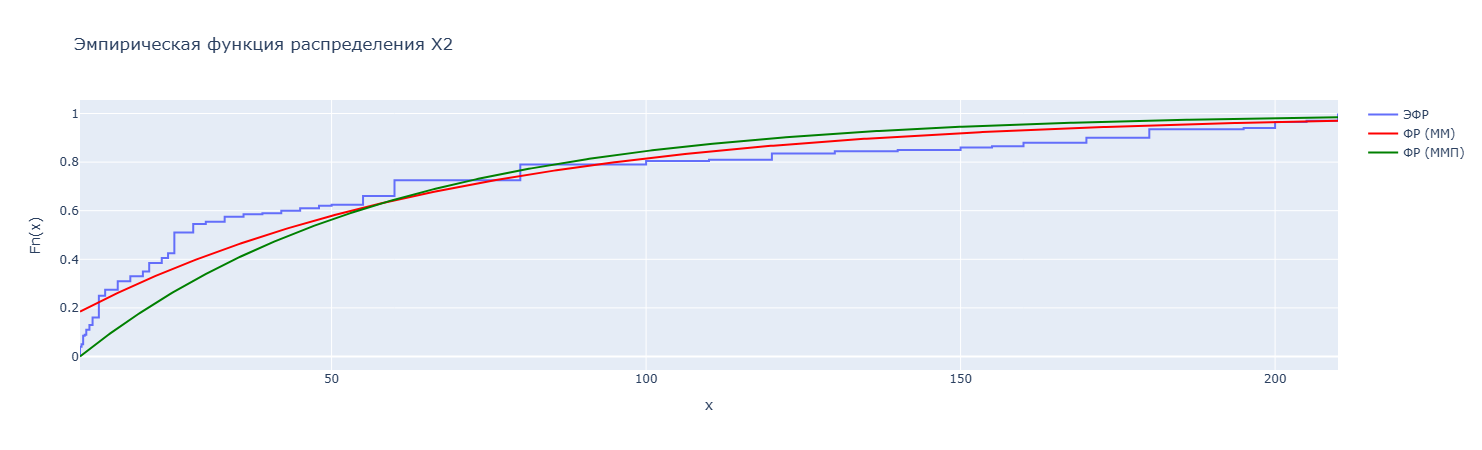
\includegraphics[width=0.85\textwidth]{plots/fit_x2.png}
\caption{$X_2$: сравнение ЭФР с теоретическими ФР (ММ и ММП)}
\end{figure}

\subsection{$X_3$: равномерное $U(a, b)$}

\textbf{Метод моментов:} $\hat a = \bar x - \sqrt{3}S = -1.89$, $\hat b = \bar x + \sqrt{3}S = 101.92$.

\textbf{ММП:} $L(a,b) = 1/(b-a)^n$ --- максимизируется при минимальном $(b-a)$ $\Rightarrow$ $\hat a = \min(x_i) = 0$, $\hat b = \max(x_i) = 99$.

\begin{figure}[H]
\centering
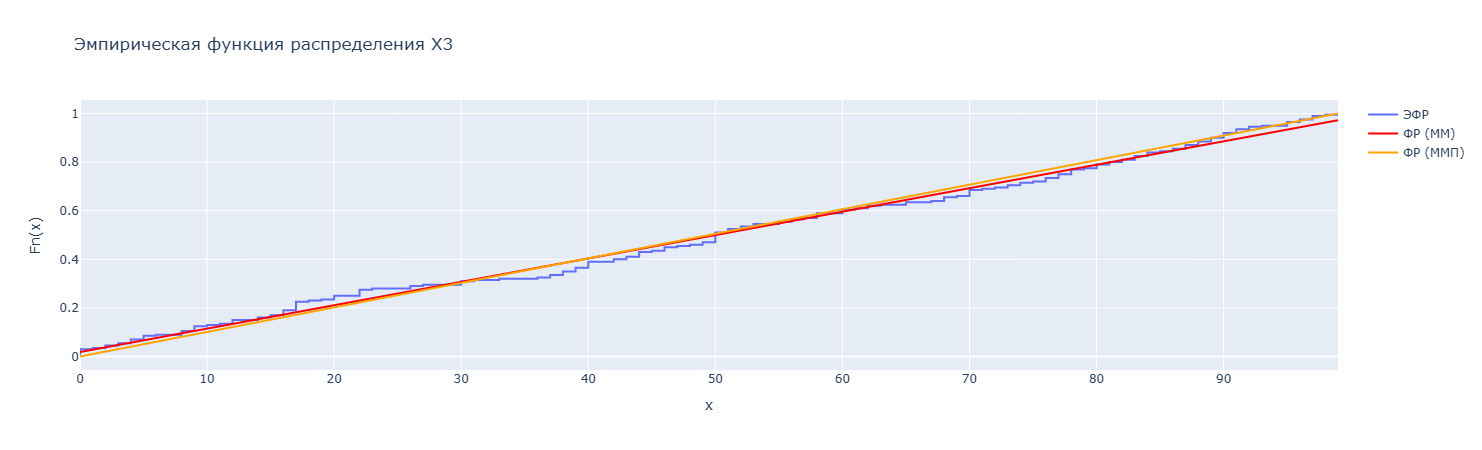
\includegraphics[width=0.85\textwidth]{plots/fit_x3.png}
\caption{$X_3$: сравнение ЭФР с теоретическими ФР (ММ и ММП)}
\end{figure}

% ============ 4.4 ============
\section{Оценивание параметрической вероятности (п. 4.4)}

Порог $x_0 = \bar x + \hat\sigma$. Оценка $P(X > x_0)$:

\begin{table}[H]
\centering
\caption{Сравнение эмпирической и параметрической оценок $P(X > x_0)$}
\begin{tabular}{lcccc}
\toprule
& $x_0$ & Эмпирическая & Параметрическая & Расхождение \\
\midrule
$X_1$ & $0.0121$ & $0.1250$ & $0.1587$ & $0.0337$ \\
$X_2$ & $118.98$ & $0.1900$ & $0.1043$ & $0.0857$ \\
$X_3$ & $79.98$ & $0.2250$ & $0.1921$ & $0.0329$ \\
\bottomrule
\end{tabular}
\end{table}

Расхождения умеренные: для $X_1$ и $X_3$ малы, для $X_2$ чуть больше из-за тяжёлого хвоста реальных данных.

% ============ 4.5 ============
\section{Моменты по сгруппированной выборке (п. 4.5)}

Формулы:
$$\hat X_g = \frac{1}{n}\sum_{k=1}^{m} n_k \hat X_k, \qquad \hat\sigma^2_g = \frac{1}{n-1}\sum_{k=1}^{m} n_k (\hat X_k - \hat X_g)^2$$

\begin{table}[H]
\centering
\caption{Сравнение оценок по исходным и сгруппированным данным}
\begin{tabular}{lcccc}
\toprule
& $\hat{EX}$ (исходн.) & $\hat{EX}$ (групп.) & $\hat{DX}$ (исходн.) & $\hat{DX}$ (групп.) \\
\midrule
$X_1$ & $0.000071$ & $\approx 0.000071$ & $0.000145$ & $\approx 0.000145$ \\
$X_2$ & $58.22$ & $\approx 58$ & $3692.08$ & $\approx 3700$ \\
$X_3$ & $50.02$ & $\approx 50$ & $898.18$ & $\approx 900$ \\
\bottomrule
\end{tabular}
\end{table}

Отклонения малы. Потеря точности связана с заменой значений серединами интервалов.

% ============ 4.6 ============
\section{Доверительные интервалы (п. 4.6)}

Уровень доверия $1 - \alpha = 0.95$.

\subsection{Асимптотический ДИ для $EX$ (по ЦПТ)}

$$EX \in \left(\bar x - z_{1-\alpha/2}\frac{\hat\sigma}{\sqrt{n}},\; \bar x + z_{1-\alpha/2}\frac{\hat\sigma}{\sqrt{n}}\right)$$

\begin{table}[H]
\centering
\caption{Асимптотические доверительные интервалы для $EX$}
\begin{tabular}{lccc}
\toprule
& Нижняя граница & Верхняя граница & Ширина \\
\midrule
$X_1$ & $-0.001595$ & $0.001737$ & $0.003332$ \\
$X_2$ & $49.80$ & $66.64$ & $16.84$ \\
$X_3$ & $45.86$ & $54.17$ & $8.31$ \\
\bottomrule
\end{tabular}
\end{table}

\subsection{Точные ДИ для $X_1$ (нормальное распределение)}

Для $\mu$ при неизвестной $\sigma^2$ ($t$-распределение):
$$\mu \in \left(\bar x \pm t_{1-\alpha/2, n-1}\frac{\hat\sigma}{\sqrt{n}}\right) = (-0.001605;\; 0.001747)$$

Для $\sigma^2$ ($\chi^2$-распределение):
$$\sigma^2 \in \left(\frac{(n-1)\hat\sigma^2}{\chi^2_{1-\alpha/2}},\; \frac{(n-1)\hat\sigma^2}{\chi^2_{\alpha/2}}\right) = (0.00011985;\; 0.00017771)$$

\subsection{Интерпретация}

Доверительный интервал 95\% означает: если повторить эксперимент многократно, то в 95\% случаев построенный интервал накроет истинное значение параметра. Это \textbf{не} вероятность того, что параметр лежит в данном конкретном интервале --- параметр фиксирован, а интервал случаен.

Асимптотический и точный ДИ для $X_1$ практически совпадают --- при $n = 200$ квантили $t$-распределения уже очень близки к квантилям стандартного нормального.

% ============ 4.7 ============
\section{Итоговый вывод (п. 4.7)}

\textbf{$X_1$} (лог-доходности IMOEX) --- нормальное распределение $N(\hat\mu, \hat\sigma)$. Гистограмма колоколообразная, ЭФР S-образная, асимметрия $\approx 0$. Оценки ММ и ММП совпали.

\textbf{$X_2$} (ставка рефинансирования ЦБ РФ) --- экспоненциальное со сдвигом $Exp(\hat\lambda, \hat c)$. Выраженная правая асимметрия, нижняя граница $\approx 10\%$. Оценки ММ и ММП различаются по параметру сдвига.

\textbf{$X_3$} (копейки цены SBER) --- равномерное распределение $U(0, 99)$. Плоская гистограмма, линейная ЭФР. ММП даёт более точные границы ($[0, 99]$), чем ММ ($[-1.89, 101.92]$).

Доверительные интервалы при $n = 200$ достаточно узкие. Эмпирические и параметрические оценки $P(X > x_0)$ расходятся незначительно, что подтверждает корректность выбранных моделей.

% ============ БОНУС ============
\section{Бонус: бимодальность и кластеризация $X_4$}

\begin{figure}[H]
\centering
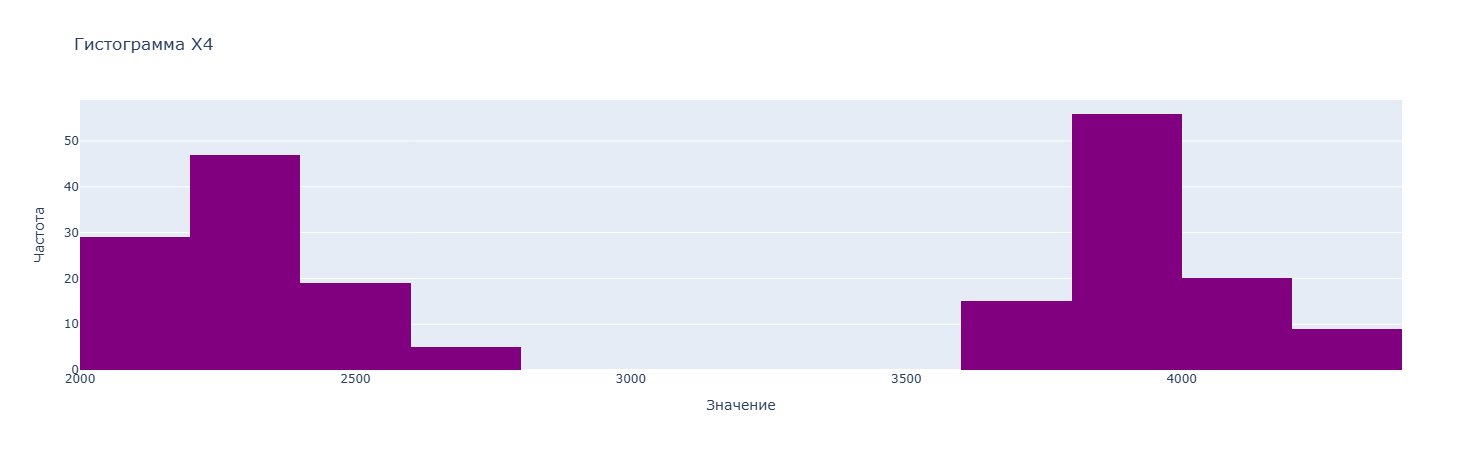
\includegraphics[width=\textwidth]{plots/overview1.png}
\caption{$X_4$: гистограмма --- два выраженных пика}
\end{figure}

\begin{figure}[H]
\centering
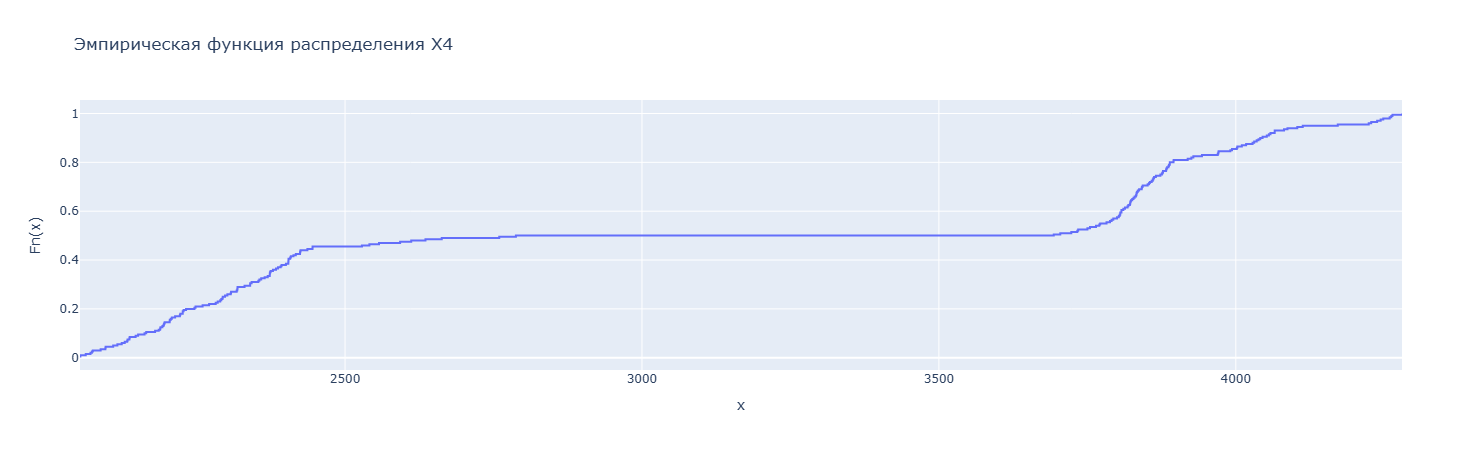
\includegraphics[width=\textwidth]{plots/overview2.png}
\caption{$X_4$: ЭФР --- два выраженных пика}
\end{figure}

Гистограмма $X_4$ имеет два пика: $\approx 2000$--$2500$ (после кризиса) и $\approx 3500$--$4200$ (до кризиса). ЭФР имеет <<ступеньку>> посередине.

Кластеризация $k$-средних ($k=2$):

\begin{table}[H]
\centering
\caption{Характеристики кластеров $X_4$}
\begin{tabular}{lccc}
\toprule
& $n$ & Среднее & Стд. откл. \\
\midrule
Кластер 0 (после кризиса) & 100 & 2300.2 & 152.7 \\
Кластер 1 (до кризиса) & 100 & 3920.8 & 145.9 \\
\midrule
Общее & 200 & 3110.5 & --- \\
\bottomrule
\end{tabular}
\end{table}

\begin{figure}[H]
\centering
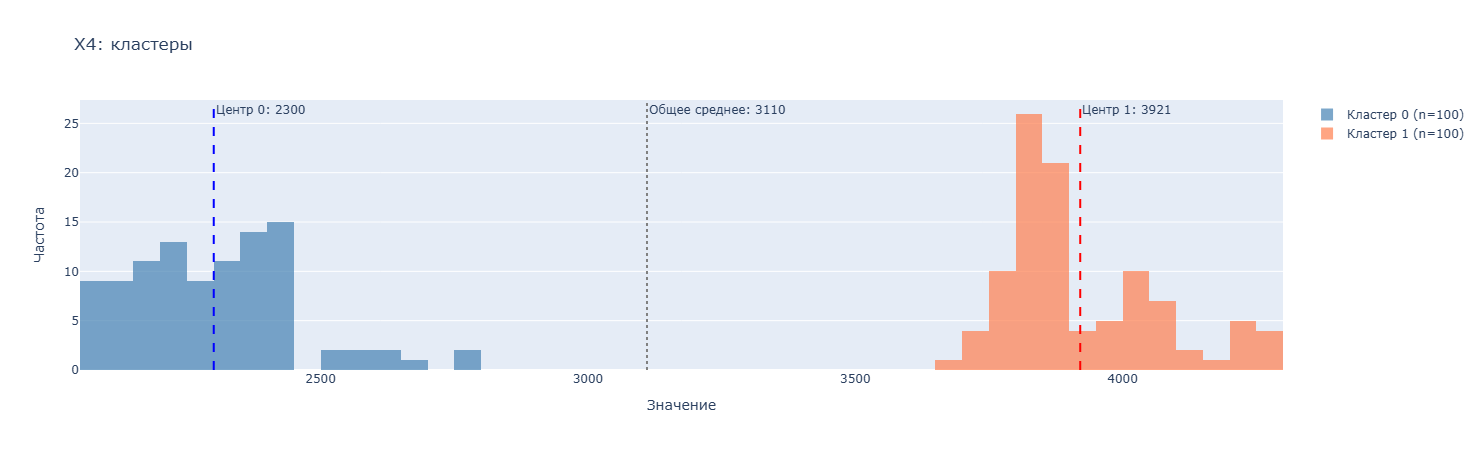
\includegraphics[width=\textwidth]{plots/clusters1.png}
\caption{$X_4$: гистограммы кластеров}
\end{figure}

\begin{figure}[H]
\centering
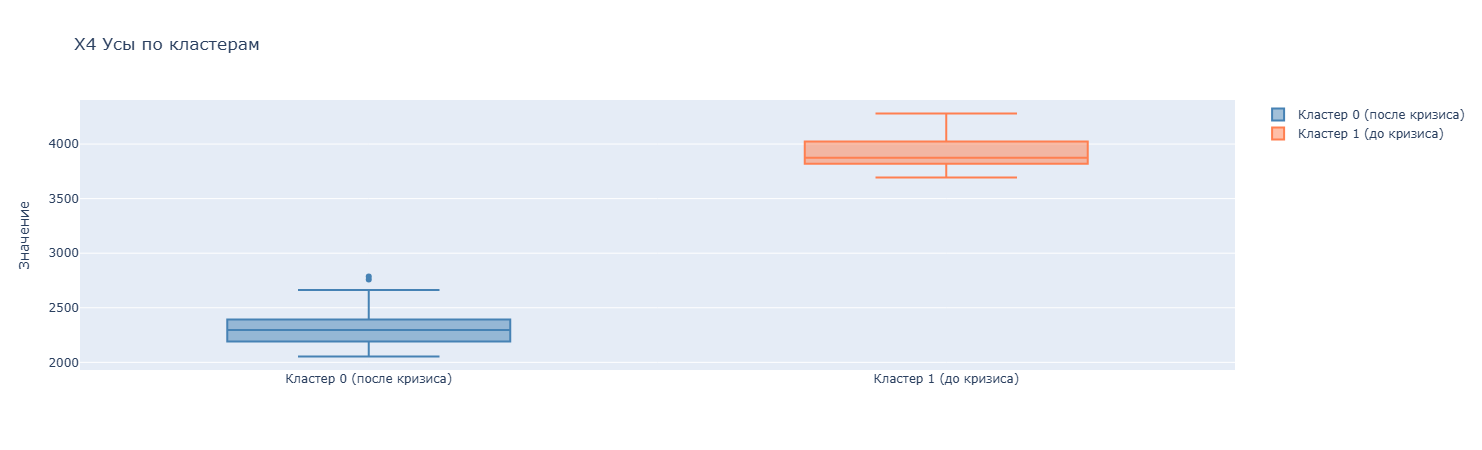
\includegraphics[width=\textwidth]{plots/clusters2.png}
\caption{$X_4$: боксы-усы}
\end{figure}

Общее среднее $\bar x = 3110$ не соответствует ни одному из режимов --- оно оказывается между двумя модами. Это <<средняя температура по больнице>>. Каждый кластер по отдельности хорошо описывается нормальным распределением.

\end{document}
